\subsection{豪斯多夫空间的子空间与积}

豪斯多夫空间 X 的子空间 A 是豪斯多夫的，这可由把第 1 目命题 5 应用于典范单射 A → X 看出。反之，我们有

命题 6. 若拓扑空间 X 的每一点都有一个闭邻域，它是 X 的豪斯多夫子空间，则 X 是豪斯多夫的。

设 \(x \in X\)，并设 \(V\) 是 \(x\) 在 \(X\) 中的一个闭邻域，使得子空间 \(V\) 是豪斯多夫的。则 \(x\) 在 \(V\) 中的诸闭邻域之交为 \(\{x\}\)（公理 \((H^i)\)）；但它们也是 \(x\) 在 \(X\) 中的闭邻域（\(\S 3, no. 1\)），因此 \(X\) 满足 \((H^i)\)。

\pandocbounded{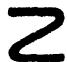
\includegraphics[keepaspectratio]{images/part001_a9a6e172.jpg}}

存在这样的非豪斯多夫空间，其中每一点都有一个豪斯多夫邻域（习题 7）。

命题 7. 豪斯多夫空间的每个积都是豪斯多夫的。反之，若非空空间的积是豪斯多夫的，则每个因子都是豪斯多夫空间。

设 \(X = \prod_{i \in I} X_i\) 是拓扑空间的一个积。于是，若 \(x, y\) 是 \(X\) 的两个不同的点，则 \(\text{pr}_i x \neq \text{pr}_i y\) 对某个指标 \(i\) 成立，而第 1 目命题 5 表明，\(X\) 是豪斯多夫的，只要诸 \(X_i\) 是豪斯多夫的。反之，若 \(X\) 是豪斯多夫的且诸 \(X_i\) 非空，则每个 \(X_i\) 同胚于 \(X\) 的一个子空间（\(\S 4\)，第 2 目，命题 4），因而是豪斯多夫的。

推论 1. 设 X 是一个集合，\((\mathbf{Y}_{\iota})_{\iota \in \mathbf{I}}\) 是豪斯多夫拓扑空间的一个族，且对每个 \(\iota \in I\)，设 \(f_{\iota}\) 是 X 到 \(Y_{\iota}\) 中的一个映射。设 X 带有最粗拓扑 \(\mathfrak{T}\)，使诸 \(f_{\iota}\) 连续。则 X 为豪斯多夫的一个必要充分条件是：对 X 的每对不同的点 x, y，\(f_{\iota}(x) \neq f_{\iota}(y)\) 对某个指标 \(\iota \in I\) 成立。

该条件依据第 1 目命题 5 是充分的。反之，设 X 是豪斯多夫的；令 \(Y = \prod_{\iota \in I} Y_{\iota}\)，并令 \(f = (f_{\iota})_{\iota \in I}\) 为映射 \(x \to (f_{\iota}(x))\)。由上面的命题 7，Y 是豪斯多夫的；又由 §4 第 1 目命题 3，\(\mathfrak{T}\) 是 Y 的拓扑在 f 下的逆像。若对 X 的两个不同的点 x, y 有 \(f(x) = f(y)\)，则显然每个（拓扑 \(\mathfrak{T}\) 中的）包含 x 的开集也包含 y，这与 X 是豪斯多夫的假设相矛盾。

推论 2. 设 \((\mathbf{X}_{\alpha}, f_{\alpha \beta})\) 是拓扑空间的一个逆系统。若诸 \(\mathbf{X}_{\alpha}\) 是豪斯多夫的，则 \(\mathbf{X} = \varprojlim \mathbf{X}_{\alpha}\) 是豪斯多夫的，并且是 \(\prod_{\alpha} \mathbf{X}_{\alpha}\) 的一个闭子空间。

第一个断言由 X 是豪斯多夫空间 \(\prod_{\alpha} X_{\alpha}\) 的子空间（命题 7）这一事实得出。为证 X 在积空间中是闭的，设 \(F_{\alpha\beta} (\alpha \leqslant \beta)\) 是 \(\prod_{\alpha} X_{\alpha}\) 中由使 \(\operatorname{pr}_{\alpha}x = f_{\alpha\beta}(\operatorname{pr}_{\beta}x)\) 的点 x 组成的子集；诸 \(F_{\alpha\beta}\) 在 \(\prod_{\alpha} X_{\alpha}\) 中是闭的（第 1 目，命题 2），因此它们的交 X 也是闭的。

显然，豪斯多夫空间的任意和（§ 2，第 4 目，例 3）都是豪斯多夫空间。

